\documentclass[a4paper, 12pt]{article}

\usepackage[utf8]{inputenc}
\usepackage[T1]{fontenc}
\usepackage{bm}						% Typesetting matrices
\usepackage{authblk}				% Affiliation in title
\usepackage{amsmath}				% All kinds of shit
\usepackage{amssymb}				% For blackboard bold
\usepackage{commath}				% Differetial operators
\usepackage{array}					% Fancy tables
\usepackage{units}					% Slanted fractions
\usepackage{enumitem}				% Sep options
\usepackage{fouridx}				% Pre-superscript
\usepackage{float}					% Force float placement
\usepackage{graphicx}				% For images etc.
\usepackage[hidelinks]{hyperref}	% Clickable toc
\usepackage[usenames, dvipsnames]{xcolor}
\newcommand{\comment}[1]{\textcolor{RedOrange}{#1}}

\title{Summary of \\ TTK4130 Modeling and Simulation}
\author{Morten Fyhn Amundsen}
\affil{NTNU}

\begin{document}
\maketitle
\tableofcontents
\newpage

\newcommand{\enforall}{\enskip \forall \enskip}
\newcommand{\residual}{\operatornamewithlimits{Res}}
\newcommand{\V}[1]{\mathbf{#1}}							% Bold vector
\newcommand{\M}[1]{\bm{#1}}								% Matrix
\newcommand{\I}{\mathbf{I}}								% Identity matrix
\newcommand{\y}{\V{y}}									% y vector
\newcommand{\ydot}{\V{\dot{y}}}							% ydot vector
\newcommand{\R}{\M{R}}									% Rotation matrix
\newcommand{\T}{^{\text{T}}}							% Transpose
\newcommand{\half}{\nicefrac{1}{2}}						% Slanted 1/2 fraction
\newcommand{\nf}[2]{\nicefrac{#1}{#2}}					% Shorthand for slanted fractions
\newcommand{\angvel}{\boldsymbol{\omega}}
\newcommand{\gv}[1]{\boldsymbol{#1}}
\newcommand{\lagr}{\mathcal{L}}
\newcommand{\presuper}[1]{\fourIdx{#1}{}{}{}}

\renewcommand{\c}{\operatorname{c}}						% Shorthand for cos, used in large matrices
\newcommand{\s}{\operatorname{s}}						% Ditto sin
\renewcommand{\b}[1]{\textbf{#1}}

%%%%%%%%%%%%%%%%%%%%%%%%%%%%%%%%%%%%%%%%%%%%%%%%%%%%%%%%%%%%
\section{Introduction}
%%%%%%%%%%%%%%%%%%%%%%%%%%%%%%%%%%%%%%%%%%%%%%%%%%%%%%%%%%%%
I can't be bothered to write much here. You know what you're doing.

\subsection{Todo}
\begin{itemize}
	\item Force and torque matrices \( \M{F}^b_{bc} \).
	\item \comment{p. 533}
\end{itemize}

%%%%%%%%%%%%%%%%%%%%%%%%%%%%%%%%%%%%%%%%%%%%%%%%%%%%%%%%%%%%
\section{Things that ought to be obvious}
%%%%%%%%%%%%%%%%%%%%%%%%%%%%%%%%%%%%%%%%%%%%%%%%%%%%%%%%%%%%
\paragraph{Eigenvalues} Values of \( \lambda \) such that: \( \det{\lambda \I - \M{A}} = 0 \).
\paragraph{Eigenvectors} Vectors \( \V{v} \) such that: \( (\M{A} - \lambda \I)\V{v} = 0 \).
\paragraph{Differentiation of \(x^2\):} \(\od{x^2}{t} = 2 \dot{x} x\)
\paragraph{Relation of velocity to ang. vel.:} \(v = r \omega\)
\paragraph{Matrix transposes:} \( (\M{A} + \M{B})\T = \M{A}\T + \M{B}\T, \quad (\M{AB})\T = \M{B}\T \M{A}\T \)
\paragraph{Inverse of \(2 \times 2\) matrix:}
\[
\M{A}^{-1} = 
\begin{pmatrix} a & b \\ c & d \end{pmatrix}^{-1} =
\frac{1}{\det \M{A}} \begin{pmatrix} d & -b \\ -c & a \end{pmatrix}
\] 

%%%%%%%%%%%%%%%%%%%%%%%%%%%%%%%%%%%%%%%%%%%%%%%%%%%%%%%%%%%%
\section{Energy-flow modelling (19)}
%%%%%%%%%%%%%%%%%%%%%%%%%%%%%%%%%%%%%%%%%%%%%%%%%%%%%%%%%%%%
A modular, rather than monolithic approach to modelling a dynamic system. Modules are connected with one \emph{potential} and one \emph{flow} variable, similar to their physical connection. At a connection, potentials must be equal, and flows must sum to zero.

\begin{table}[H]
\small
\begin{tabular}{llll}
	\b{Domain}  & \b{Potential}           & \b{Flow}                                 & \b{Result} \\
	\hline
	Translation & Velocity [m/s]          & Force [N]                                & Power [W]  \\
	Rotation    & Angular velocity [/s]   & Torque [Nm]                              & Power [W]  \\
	Electrical  & Voltage [V]             & Current [A]                              & Power [W]  \\
	Magnetic    & Mag.mot. force [A]      & Mag. flux rate [V]                       & Power [W]  \\
	Hydraulic   & Pressure [Pa]           & Volume flow rate [m\(^3\)/s]             & Power [W]  \\
	Thermal     & Temperature [K]         & Heat flow rate [J/Ks]                    & Power [W]  \\
	Chemical    & Chem. potential [J/mol] & Molar flow rate [mol/s]                  & Power [W]
\end{tabular}
\end{table}

%%%%%%%%%%%%%%%%%%%%%%%%%%%%%%%%%%%%%%%%%%%%%%%%%%%%%%%%%%%%
\section{Energy (\emph{Lyapunov}) functions and passivity (46)}
%%%%%%%%%%%%%%%%%%%%%%%%%%%%%%%%%%%%%%%%%%%%%%%%%%%%%%%%%%%%
\paragraph{Energy functions} describe the change of internal `energy' in a system. \emph{Decreasing energy implies stability.}

The time derivative of the energy function is
\begin{equation}
	\dot{V} = \pd{V}{t} + \pd{V}{\V{x}} \V{f}(\V{x}, \V{u}, t).
\end{equation}

\paragraph{Passivity} describes whether a system produces energy to its surroundings.
(Example: Power in a resistor: \(P = u i = R i^2 \implies P \geq 0 \implies\) Passive!)
\begin{itemize}
	\item Connected stable systems are not always stable...
	\item Connected passive systems are always passive, and therefore stable!
\end{itemize}
A system with input \(u\) and output \(y\) is passive if
\begin{equation}
	\int_0^t y(\tau) u(\tau) \dif \tau \geq - E_0 \enforall t \geq 0
\end{equation}
for all inputs.

\subsection{Positive realness of a transfer function (56)}
A system is passive iff its transfer function is positive real.
\paragraph{Definition:} The t.f. \(H(s)\) (rational or not) is positive real if:
\begin{enumerate}
	\item \(H(s)\) is analytic \( \enforall \Re[s] > 0 \)
	\item \(H(s)\) is real for all positive and real \(s\).
	\item \(\Re[H(s)] \geq 0 \enforall \Re [s] > 0\).
\end{enumerate}
But this is easier to use:
\paragraph{Theorem:} A rational, proper t.f. \(H(s)\) is positive real iff:\footnote{if and only if}
\begin{enumerate}
	\item \( H(s) \) has no poles in the right half plane.
	\item \( \Re[H(\jmath \omega)] \geq 0 \enforall \omega \) such that \( \jmath \omega \) is not a pole of \( H(s) \).
	\item If \( \jmath \omega_0 \) is a pole in \( H(s) \), it is a simple pole, and the residual in \( s = \jmath \omega_0 \) is positive and real, i.e.,
	\[ \residual_{s = \jmath \omega_0} H(s) = \lim_{s \to \jmath \omega_0} (s - \jmath \omega_0) H(s) > 0 \] (And some stuff about poles at infinity.)
\end{enumerate}

%%%%%%%%%%%%%%%%%%%%%%%%%%%%%%%%%%%%%%%%%%%%%%%%%%%%%%%%%%%%
\section{Simulation (509)}
%%%%%%%%%%%%%%%%%%%%%%%%%%%%%%%%%%%%%%%%%%%%%%%%%%%%%%%%%%%%
\subsection{Notation (517)}
\begin{equation}\label{eq:ivp}
	\underbrace{
		\underbrace{
			\V{\ydot} = \V{f}(\y, t)
		}_{
			\text{ODE}
		}
		,\quad \y(t_0) = \y_0
	}_{\text{IVP}}
\end{equation}
Given this, we want to approximate \( \V{y}(t) \).

\subsection{Error (517)}
The \emph{local solution} \( \y_L(t_n; t) \) is the exact solution of \eqref{eq:ivp} with initial condition \( \y_n \) at time \( t_n \):
\begin{equation}
	\ydot_L(t_n; t) = \V{f}[\y_L(t_n; t)], \quad \y_L(t_n; t_n) = \y_n
\end{equation}
I.e., if the system really is in state \( \y_n \) at time \( t_n \), the local solution is the true behaviour.

This lets us define the \emph{local error}: the difference between the computed solution and the local solution at \( t_{n+1} \):
\begin{equation}
	\V{e}_{n+1} = \y_{n+1} - \y_L(t_n; t_{n+1})
\end{equation}

The \emph{global error} is the difference between the computed solution and the exact solution at \( t_{n+1} \):
\begin{equation}
	\V{E}_{n+1} = \y_{n+1} - \y(t_{n+1})
\end{equation}

\subsection{Order of a one-step method (517)}
A method is of order \( p \) if \( \V{e}_{n+1} = O(h^{p+1}) \).

Given the IVP in \eqref{eq:ivp} and a one-step method (of step length \( h \))
\begin{equation}\label{eq:onestep}
	\y_{n+1} = \y_n + h \phi(\y_n, t_n),
\end{equation}
if then
\begin{equation}
	\y_{n+1} = \y_n + h \V{f}(\y_n, t) + \frac{h^2}{2} \od{\V{f}(\y_n, t)}{t} + \hdots + \frac{h^p}{p!} \od[p-1]{\V{f}(\y_n, t)}{t} + O(h^{p+1})
\end{equation}
holds, the local error is \( O(h^{p+1}) \) and the method is of order \( p \).

\subsection{Linearisation (518)}
The linearisation of \eqref{eq:ivp} around \( \y^* \) is
\begin{equation}
	\Delta \ydot = \M{J} \Delta \y,
\end{equation}
where \( \M{J} \) is
\begin{equation}
	\M{J}
	= \pd{\V{f}(\y,t)}{\y} \biggr\rvert_{\y = \y^*}
	= \left\{ \dpd{f_i(\y,t)}{y_j} \biggr\rvert_{\y = \y^*} \right\}.
\end{equation}

\subsection{Stability (531)}
\subsubsection{Scalar test system}
Given the scalar test system
\begin{equation}
	\dot{y} = \lambda y
\end{equation}
we get
\begin{equation}
	y_{n+1} = R(h \lambda) y_n
\end{equation}
where \( R(h \lambda )\) is the stability function of a numerical method.
\subsubsection{Requirement for stability}
The numerical solution \( \Delta \y_n \) of the linearised system is stable if:
\begin{equation}
	| R(h\lambda_i) | \leq 1
\end{equation}
for all eigenvalues \( \lambda_i \) of \( \M{J} \).

\subsection{Explicit Runge-Kutta methods (ERK) (526)}
Given the IVP in \eqref{eq:ivp} and the generic one-step method in \eqref{eq:onestep}, the general ERK is
\begin{equation}
	\begin{aligned}
		\V{k}_1 &= \V{f}(\y_n, \enspace t_n) \\
		\V{k}_2 &= \V{f}(\y_n + h a_{21}\V{k}_1, \enspace t_n + c_2 h) \\
		\V{k}_3 &= \V{f}(\y_n + h (a_{31}\V{k}_1 + a_{32} \V{k}_2), \enspace t_n + c_3 h) \\
				& \enspace \vdots \\
		\V{k}_\sigma &= \V{f}(\y_n + h (a_{\sigma 1}\V{k}_1 + \hdots + a_{\sigma,\sigma-1}\V{k}_{\sigma-1}), \enspace t_n + c_\sigma h) \\
		\y_{n+1} &= \y_n + h (b_1 \V{k}_1 + \hdots + b_\sigma \V{k}_\sigma).
	\end{aligned}
\end{equation}
The weights can be arranged in a \emph{Butcher array}:
\begin{equation}
\begin{array}{c|ccccc}
0        &              &              &        &                      &          \\
c_2      & a_{21}       &              &        &                      &          \\
c_3      & a_{31}       & a_{32}       &        &                      &          \\
\vdots   & \vdots       & \vdots       & \ddots &                      &          \\
c_\sigma & a_{\sigma 1} & a_{\sigma 2} & \hdots & a_{\sigma, \sigma-1} &          \\ \hline
         & b_1          & b_2          & \hdots & b_{\sigma-1}         & b_\sigma \\
\end{array}
\quad \text{or} \quad
\begin{array}{c|c}
    \V{c} & \M{A}   \\ \hline
          & \V{b}\T \\
\end{array}
\end{equation}
Where \( \sigma \) is the number of stages.

\subsubsection{ERK stability}
The stability function of an ERK is
\begin{equation}
	R_E(h\lambda) = \det \left[ \I -\lambda h \left( \M{A} - \V{1 b}\T \right) \right]
\end{equation}
where \(\M{A}\) and \(\V{b}\) are given by the Butcher array.

For ERKs of order \( p = \sigma \leq 4 \):
\begin{equation}
	R_E(h \lambda) = 1 + h \lambda + \dots + \frac{h^p \lambda^p}{p!}
\end{equation}
Valid for Euler's method, Modified Euler, RK4, and at least one other. These are the methods that are actually used.

\subsubsection{Euler's method (Forward Euler)}
\begin{equation}
	\y_{n+1} = \y_n + h\V{f}(\y_n, t_n)
	\iff
	\begin{array}{c|c}
		0 &   \\ \hline
		  & 1 \\
	\end{array}
\end{equation}

\subsubsection{Improved Euler}
\begin{equation}
	\begin{array}{rcl}
		\V{k}_1  &=& \V{f}(\y_n, t_n) \\
		\V{k}_2  &=& \V{f}(\y_n + h \V{k}_1, t_n + h) \\
		\y_{n+1} &=& \y_n + \frac{h}{2}(\V{k}_1 + \V{k}_2) \\
	\end{array}
	\iff
	\begin{array}{c|cc}
		0 &       &       \\
		1 & 1     &       \\ \hline
		  & \half & \half \\
	\end{array}
\end{equation}

\subsubsection{Modified Euler (Explicit midpoint)}
\begin{equation}
	\begin{array}{rcl}
		\V{k}_1  &=& \V{f}(\y_n, t_n) \\
		\V{k}_2  &=& \V{f}(\y_n + \frac{h}{2}\V{k}_1, t_n + \frac{h}{2}) \\
		\y_{n+1} &=& \y_n + h\V{k}_2 \\
	\end{array}
	\iff
	\begin{array}{c|cc}
		0     &       &   \\
		\half & \half &   \\ \hline
		      & 0     & 1 \\
	\end{array}
\end{equation}

\subsubsection{Heun's method}
\begin{equation}
	\begin{array}{c|ccc}
		0         &           &           &           \\
		\nf{1}{3} & \nf{1}{3} &           &           \\
		\nf{2}{3} & 0         & \nf{2}{3} &           \\
		\hline
		          & \nf{1}{4} & 0         & \nf{3}{4} \\
	\end{array}
\end{equation}

\subsubsection{Runge-Kutta 4}
\begin{equation}
    \begin{array}{c|cccc}
		0     &           &           &           &           \\
		\half & \half     &           &           &           \\
		\half & 0         & \nf{1}{2} &           &           \\
		1     & 0         & 0         & 1         &           \\ \hline
              & \nf{1}{6} & \nf{2}{6} & \nf{2}{6} & \nf{1}{6} \\
    \end{array}
\end{equation}

\subsection{Implicit Runge-Kutta methods (IRK) (534)}
Defined as
\begin{equation}
\begin{aligned}
\V{k}_1      &= \V{f}(\y_n + h(a_{11}\V{k}_1 + \hdots + a_{1 \sigma}\V{k}_\sigma), \enspace t_n + c_1 h) \\
             &  \enskip \vdots \\
\V{k}_\sigma &= \V{f}(\y_n + h(a_{\sigma 1}\V{k}_1 + \hdots + a_{\sigma \sigma}\V{k}_\sigma), \enspace t_n + c_\sigma h) \\
\y_{n+1}     &= \y_n + h (b_1\V{k}_1 + \hdots + b_\sigma\V{k}_\sigma)
\end{aligned}
\end{equation}

\begin{equation}
\begin{array}{c|ccccc}
c_1      & a_{11}       & a_{12}       & \dots  & \dots               & a_{1\sigma}      \\
c_2      & a_{21}       & a_{22}       & \dots  & \dots               & a_{1\sigma}      \\
\vdots   & \vdots       & \vdots       & \ddots & \ddots              & \vdots           \\
c_\sigma & a_{\sigma 1} & a_{\sigma 2} & \dots  & a_{\sigma,\sigma-1} & a_{\sigma\sigma} \\ \hline
         & b_1          & b_2          & \dots & b_{\sigma-1}         & b_\sigma         \\
\end{array}
\quad \text{or} \quad
\begin{array}{c|c}
    \V{c} & \M{A}   \\ \hline
          & \V{b}\T \\
\end{array}
\end{equation}
IRKs efficiently solve stiff systems (i.e. systems with a large spread in eigenvalues). ERKs do not. Stability is generally the motivation for using IRKs, not accuracy.

\subsubsection{IRK stability}
The stability of an IRK is given by
\begin{align}
	R(h\lambda)	&= 1 + \lambda h \V{b}\T ( \I - h \lambda \M{A} )^{-1} \V{1} \\
				&= \frac{
					\det \left( \I - \lambda h \left[ \M{A} - \V{1b}\T \right] \right)
					}{
					\det ( \I - \lambda h \M{A} )
					}
\end{align}

\subsubsection{Implicit Euler (Radau IIA)}
\begin{equation}
	\begin{array}{rcl}
		\V{k}_1  &=& \V{f}(\y_n + h \V{k}_1, t_{n+1}) \\
		\y_{n+1} &=& \y_n + h \V{k}_1 \\
	\end{array}
	\iff
	\begin{array}{c|c}
		1 & 1 \\ \hline
		  & 1 \\
	\end{array}
\end{equation}
This is stable for all eigenvalues \emph{outside} a unit circle with center \((1, 0)\)!

\subsection{A- and L-stability (546)}
\paragraph{A-stability:} A method is A-stable if \( |R(\lambda h)| \leq 1 \enforall \Re(\lambda) \leq 0 \).

This implies that the method is stable for all stable test systems. Thus, it is also stable for systems with very fast dynamics compared to \(h\), but note that aliasing can occur. High frequency oscillations appear in the solution as oscillations slower than the Nyquist frequency \( \frac{\pi}{h}\).

Note that no explicit methods are A-stable.

\paragraph{L-stability:} A method is L-stable if it is A-stable, and \(\lim_{\omega \rightarrow \infty} |R(\jmath \omega h)| = 0\) for all systems \( \dot{y} = \lambda y \) where \( \lambda = \jmath \omega \).

L-stable methods dampen out the inaccurate, fast dynamics that can occur with A-stable methods.

\subsection{Padé-approximations (548)}
The local solution of the test system \( \dot{y} = \lambda y \) over a time step, and the numerical solution of the same system, is
\begin{gather}
	\dot{y}_L(t_n; t_{n+1}) = e^{\lambda h} y_n \\
	y_{n+1} = R(\lambda h) y_n
\end{gather}
The accuracy of the numerical solution depends on how well \( R(\lambda h) \) approximates the exponential function.

A Padé approximation \( P^k_m(s) \) is the best rational approximation of \( e^s \) with a numerator of order \(k\) and a denominator of order \(m\).
%%%%%%%%%%%%%%%%%%%%%%%%%%%%%%%%%%%%%%%%%%%%%%%%%%%%%%%%%%%%
\section{Rotation matrices (218)}
%%%%%%%%%%%%%%%%%%%%%%%%%%%%%%%%%%%%%%%%%%%%%%%%%%%%%%%%%%%%
\subsection{Vectors (209)}
The vector
\begin{equation}
	\vec{v} = v_1 \vec{a_1} + v_2 \vec{a_2} + v_3 \vec{a_3}
\end{equation}
has `built in' information about its frame of reference (it is \emph{coordinate free}). However, the coordinate vector
\begin{equation}
	\V{u}^a =
	\begin{pmatrix}
		u_1 & u_2 & u_3 \\
	\end{pmatrix}
	\T
\end{equation}
does not, and we must indicate which frame of reference it is given in (frame \(a\) in this case).

\subsection{Skew-symmetric form (211)}
\begin{equation}
	\V{u}^\times :=
	\begin{pmatrix}
		0    & -u_3 & u_2  \\
		u_3  & 0    & -u_1 \\
		-u_2 & u_1  & 0    \\
	\end{pmatrix}
\end{equation}

\subsection{Vector cross product (211)}
\begin{equation}
	\V{w} = \V{u}^\times \V{v}
	\iff
	\vec{w} = \vec{u} \times \vec{v}
\end{equation}
Alternatively:
\begin{equation}
	\V{w} = \V{u}^\times \V{v} =
	\begin{pmatrix}
		u_2 v_3 - u_3 v_2 \\
		u_3 v_1 - u_1 v_3 \\
		u_1 v_2 - u_2 v_1 \\
	\end{pmatrix}
\end{equation}

\subsection{Properties of the rotation matrix (219)}
\paragraph{Notation:} \( \V{v}^a = \begin{pmatrix} v_1^a & v_2^a & v_3^a \end{pmatrix}\T \) is vector \( \V{v} \) given in the coordinates of \(a\).

\begin{equation}
	\begin{aligned}
		\V{v}^a				&= \R_b^a \V{v}^b \\
		\R_a^b				&= (\R_b^a)^{-1} = (\R_b^a)\T \\
		\R^a_c				&= \R^a_b \R^b_c \\
		(\V{u}^b)^\times	&= \R^b_a (\V{u}^a)^\times \R^a_b \\
	\end{aligned}
\end{equation}
\paragraph{Definition:} A matrix \(\R\) is a rotation matrix iff \(\R \in SO(3)\):
\begin{equation}
	SO(3) = \lbrace \R \enspace |
	\enspace \R \in \mathbb{R}^{3 \times 3},
	\enspace \R\T\R = \I,
	\enspace \det \R = 1 \rbrace
\end{equation}

\subsection{Simple rotations (221)}
A \emph{simple rotation} is a rotation about a fixed axis. Rotation matrices for rotation around the \( x \), \( y \), and \( z \) axes, respectively, are as follows:
\begin{gather}\label{eq:simplerot}
	\R_x(\phi) =
	\begin{pmatrix}
		1 & 0         & 0          \\
		0 & \cos \phi & -\sin \phi \\
		0 & \sin \phi & \cos \phi  \\
	\end{pmatrix} \\
	\R_y(\theta) =
	\begin{pmatrix}
		\cos \theta  & 0 & \sin \theta \\
		0            & 1 & 0           \\
		-\sin \theta & 0 & \cos \theta \\
	\end{pmatrix} \\
	\R_z(\psi) =
	\begin{pmatrix}
		\cos \psi & -\sin \psi & 0 \\
		\sin \psi & \cos \psi  & 0 \\
		0         & 0          & 1 \\
	\end{pmatrix}
\end{gather}

\subsection{Euler angles (224)}
A parametrisation of rotation about three axes. Three parameters \( \psi, \theta, \phi \). Singularities exist.
\paragraph{Roll, pitch, yaw:} A rotation \( \psi \) about the \( z \)-axis, then \( \theta \) about the (rotated) \( y \)-axis, then \( \phi \) about the (also rotated) \( x \)-axis.
\begin{equation}
	\begin{aligned}
		\R^a_b &= \R_z(\psi) \R_y(\theta) \R_{\underline{x}}(\phi) \\
		&=
		\begin{pmatrix}
			\c\psi \s\theta & \c\psi \s\theta \s\phi - \s\psi \c\phi & \s\psi \s\phi + \c\psi \s\theta \c\phi \\
			\s\psi \c\theta & \c\psi \c\phi + \s\psi \s\theta \s\phi & \s\psi \s\theta \c\phi - \c\psi \s\phi \\
			-\s\theta       & \c\theta \s\phi                        & \c\theta \c\phi                        \\
		\end{pmatrix}
	\end{aligned}
\end{equation}
\paragraph{Classical Euler angles:} A rotation \( \psi \) about the \( z \)-axis, then \( \theta \) about the (rotated) \( y \)-axis, then \( \phi \) about the (also rotated) \( z \)-axis.
\begin{equation}
	\begin{aligned}
	\R^a_b &= \R_z(\psi) \R_y(\theta) \R_{\underline{z}}(\phi) \\
	&=
	\begin{pmatrix}
		\c\psi \c\theta \c\phi - \s\psi \s\phi & -\c\psi \c\theta \s\phi - \s\psi \c\phi & \c\psi \s\theta \\
		\s\psi \c\theta \c\phi + \c\psi \s\phi & \c\psi \c\phi - \s\psi \c\theta \s\phi  & \s\psi \s\theta \\
		-\s\theta \c\phi                       & \s\theta \s\phi                         & \c\theta        \\
	\end{pmatrix}
	\end{aligned}
\end{equation}

\subsection{Angle-axis description of rotation (226)}
Describes a rotation by an axis of rotation \( \V{k} \) about which we move by an angle \( \theta \) (four parameters \( k_1, k_2, k_3, \theta \)).
\begin{equation}
	\R^a_b \V{k} = \V{k}, \quad \V{k}^a = \V{k}^b = \V{k}
\end{equation}
With this method, the rotation matrix becomes
\begin{equation}
	\R^a_b = \cos \theta \I
	+ \sin \theta (\V{k}^a)^\times
	+ (1-\cos \theta) \V{k}^a(\V{k}^a)\T
\end{equation}

\subsection{Euler parameters (231)}
The parameters
\begin{equation}
	\eta = \cos \frac{\theta}{2}, \quad
	\gv{\epsilon} = \V{k} \sin \frac{\theta}{2}
\end{equation}
lead to the rotation matrix
\begin{equation}
	\R_e(\eta, \gv{\epsilon}) = \I
	+ 2 \eta \gv{\epsilon}^\times
	+ 2 \gv{\epsilon}^\times \gv{\epsilon}^\times
	.
\end{equation}
This is nice, because:
\begin{itemize}[nosep]
	\item No singularities!
	\item No trigonometry!
	\item \( \eta^2 + \vec{\epsilon} \cdot \vec{\epsilon} = 1 \): Easy to normalise (avoid roundoff errors).
\end{itemize}

\subsection{Homogenous transformation matrices (223)}
The position and orientation of frame \( b \) relative to frame \( a \) is given by the homogenous transformation matrix
\begin{equation}
	\M{T}^a_b =
	\begin{pmatrix}
		\R^a_b  & \V{r}^a_{ab} \\
		\V{0}\T & 1
	\end{pmatrix}
	\in SE(3)
\end{equation}
where \( \V{r}^a_{ab} \) is the position of frame \( b \) relative to frame \( a \), expressed in the coordinates of frame \( a \). (Position as in position of the origin.)
The set \(SE(3)\) is defined as:
\begin{equation}
	SE(3) = \left\lbrace \M{T} \enspace |
	\enspace \M{T} = \begin{pmatrix} \R & \V{r} \\ \V{0}\T & 1 \end{pmatrix},
	\enspace \R \in SO(3),
	\enspace \V{r} \in \mathbb{R}^3
	\right\rbrace
\end{equation}

\subsection{Angular velocity (239)}
This is super funky and magical: The vector \( \angvel^a_{ab} \) defined by satisfying
\begin{equation}
	( \angvel^a_{ab} )^\times =
	\M{\dot{R}}^a_b ( \R^a_b )\T
\end{equation}
turns out to represent the angular velocity of \( b \) relative to \( a \).

Then, the kinematic differential equations for the rotation matrix is given in two forms
\begin{equation}
	\begin{aligned}
		\M{\dot{R}}^a_b &= (\angvel^a_{ab})^\times \R^a_b \\
		\M{\dot{R}}^a_b &= \R^a_b (\angvel^b_{ab})^\times
	\end{aligned}
\end{equation}

\paragraph{Example} (See \eqref{eq:simplerot} for the definition of \( \R_x \).)
\begin{equation}
	\M{\dot{R}}_x(\phi) \R_x\T(\phi) =
	\begin{pmatrix}
		0 & 0       & 0       \\
		0 & -\s\phi & -\c\phi \\
		0 &  \c\phi & -\s\phi \\
	\end{pmatrix}
	\dot{\phi}
	\underbrace{
		\begin{pmatrix}
			1 &  0      & 0      \\
			0 &  \c\phi & \s\phi \\
			0 & -\s\phi & \c\phi \\
		\end{pmatrix}
	}_{\R_x\T(\phi)}
	=
	\begin{pmatrix}
		0 & 0          & 0           \\
		0 & 0          & -\dot{\phi} \\
		0 & \dot{\phi} & 0           \\
	\end{pmatrix}
\end{equation}
which gives \( \angvel_x = \begin{pmatrix} \dot{\phi} & 0 & 0 \end{pmatrix}\T \).
Similarly, \( \angvel_y = \begin{pmatrix} 0 & \dot{\theta} & 0 \end{pmatrix}\T \)
and \( \angvel_z = \left( 0 \enskip 0 \enskip \dot{\psi} \right) \T \)

\subsubsection{Simple rotation}
Angular velocity \( \vec{\omega}_{ab} \) about the axis of rotation \( \vec{k} \) is:
\begin{equation}
	\vec{\omega}_{ab} = \dot{\theta} \vec{k}
\end{equation}

\subsubsection{Composite rotation}
Angular velocity of a composite rotation matrix \( \R^a_d = \R^a_b \R^b_c \R^c_d \)  is
\begin{equation}
	\vec{\omega}_{ad} = \vec{\omega}_{ab} + \vec{\omega}_{bc} + \vec{\omega}_{cd}
\end{equation}
which on coordinate form is
\begin{equation}
	\begin{aligned}
		\angvel^a_{ad} &= \angvel^a_{ab} +        \angvel^a_{bc} +        \angvel^a_{cd} \\
		               &= \angvel^a_{ab} + \R^a_b \angvel^b_{bc} + \R^a_b \R^b_c \angvel^c_{cd} \\
	\end{aligned}
\end{equation}

\subsubsection{Differentiation of vectors}
\begin{gather}
	\V{\dot{u}}^a = \R^a_b \left[ \V{\dot{u}}^b + (\angvel^b_{ab})^\times \V{u}^b \right] \\
	\frac{\fourIdx{a}{}{}{}\dif}{\dif t} \vec{u} = \frac{\fourIdx{b}{}{}{}\dif}{\dif t} \vec{u} + \vec{\omega}_{ab} \times \vec{u}
\end{gather}

%%%%%%%%%%%%%%%%%%%%%%%%%%%%%%%%%%%%%%%%%%%%%%%%%%%%%%%%%%%%
\section{Kinematic differential equations (244)}
%%%%%%%%%%%%%%%%%%%%%%%%%%%%%%%%%%%%%%%%%%%%%%%%%%%%%%%%%%%%
Rotational deviation cannot be described by subtraction. Instead, it is described by
\begin{equation}
	\widetilde{\R}_a := \R \R_d\T \implies \R = \widetilde{\R}_a \R_d
	, \quad \widetilde{\R}_a \in SO(3)
\end{equation}
where \( \R = \R^a_b \) is the orientation and \( \R_d \) is the desired orientation.

Then the kinematic differential equations for the deviation are
\begin{gather}
	\widetilde{\angvel}^a = \angvel^a - \angvel^a_d \\
	\dod{}{t} \widetilde{\R}_a = \left( \widetilde{\angvel}^a \right)^\times \widetilde{\R}_a
\end{gather}

\subsection{Rigid body kinematics (259)}
\subsubsection{Configuration}
\begin{figure}[H]
	\centering
	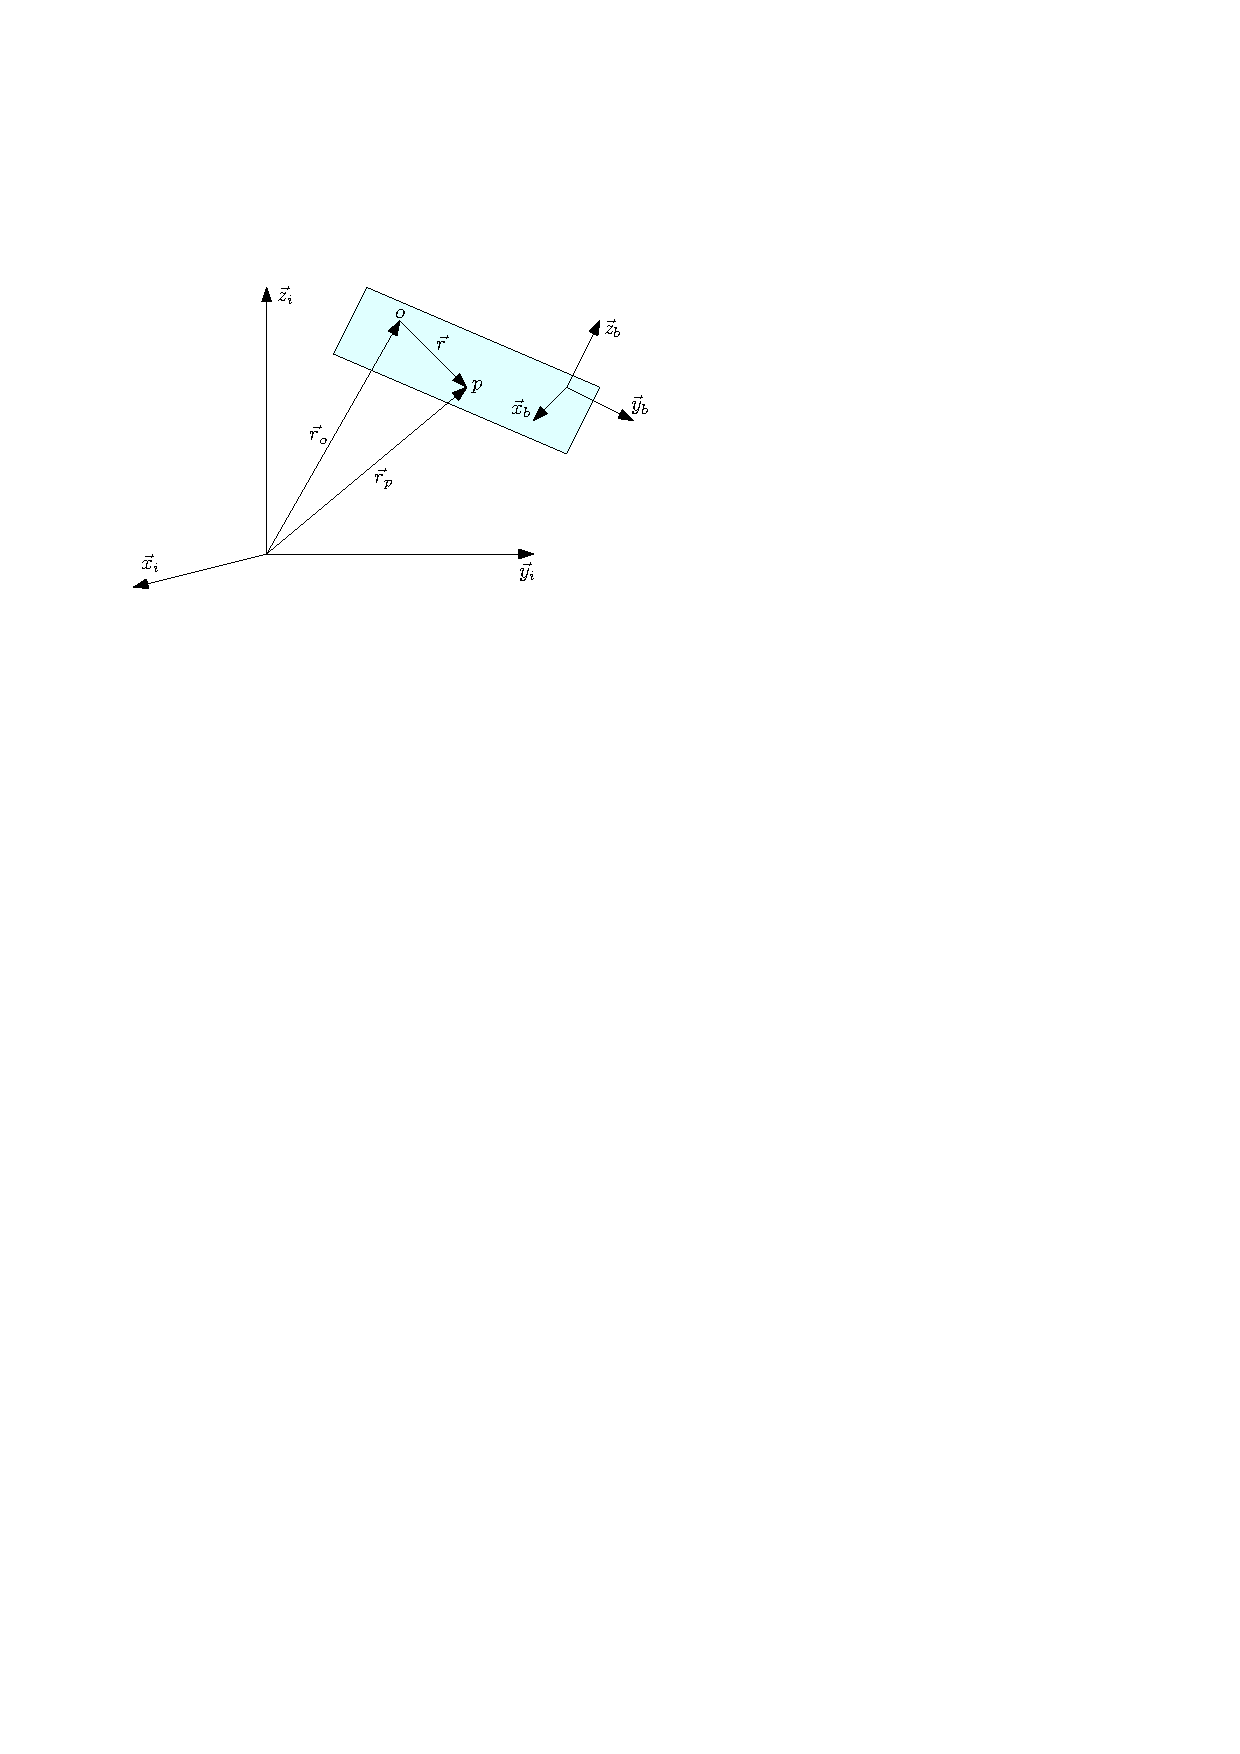
\includegraphics{rigid_body}
\end{figure}

The orientation \(\R^i_b\) of a rigid body and the position \(\vec{r}_o\) of a point \(o\) in the body, both in relation to a reference frame \(i\), define its configuration. The position of any point \(p\) in the body is given by
\begin{equation}
	\vec{r}_p = \vec{r}_o + \vec{r}.
\end{equation}
In the reference frame, \(\vec{r}\) is
\begin{equation}
	\V{r}^i = \R^i_b \V{r}^b
\end{equation}

\subsubsection{Velocity}
Definition:
\begin{equation}
	\vec{v}_o := \frac{\presuper{i}\dif}{\dif t} \vec{r}_o, \quad 
	\vec{v}_p := \frac{\presuper{i}\dif}{\dif t} \vec{r}_p
\end{equation}
Alternatively:
\begin{equation}
	\vec{v}_p = \vec{v}_o + \frac{\presuper{b} \dif}{\dif t} \vec{r} + \vec{\omega}_{ib} \times \vec{r}
\end{equation}

\subsubsection{Acceleration}
Definition (translation):
\begin{equation}
	\vec{a}_o := \frac{\presuper{i}\dif\,^2}{\dif t^2} \vec{r}_o, \quad 
	\vec{a}_p := \frac{\presuper{i}\dif\,^2}{\dif t^2} \vec{r}_p
\end{equation}
Definition (rotation):
\begin{equation}
	\vec{\alpha}_{ib} := \frac{\presuper{i}\dif\,^2}{\dif t^2} \vec{\omega}_{ib}
	= \frac{\presuper{b}\dif\,^2}{\dif t^2} \vec{\omega}_{ib}
\end{equation}
In terms of accelerion, ang. acceleration and velocities:
\begin{multline}
		\underbrace{\vec{a}_p}_{\text{Acceleration of \(p\)}} =
		\underbrace{\vec{a}_o}_{\text{Acceleration of \(o\)}} +
		\underbrace{\frac{\presuper{b}\dif\,^2}{\dif t^2} \vec{r}}_{\text{Second derivative of \(\vec{r}\) in \(b\)}} \\ +
		\underbrace{2 \vec{\omega}_{ib} \times \frac{\presuper{b}\dif}{\dif t} \vec{r} }_{\text{Coriolis acceleration}} +
		\underbrace{\vec{\alpha}_{ib} \times \vec{r}}_{\text{Transversal acceleration}} +
		\underbrace{\vec{\omega}_{ib} \times \left( \vec{\omega}_{ib} \times \vec{r} \right)}_{\text{Centripetal acceleration}}
\end{multline}
Alternatively:
\begin{equation}
	\vec{a}_p =
	\frac{\presuper{b}\dif}{\dif t} \vec{v}_o +
	\vec{\omega}_{ib} \times \vec{v}_o +
	\frac{\presuper{b}\dif\,^2}{\dif t^2} \vec{r} +
	2 \vec{\omega}_{ib} \times \frac{\presuper{b}\dif}{\dif t} \vec{r} +
	\vec{\alpha}_{ib} \times \vec{r} +
	\vec{\omega}_{ib} \times \left( \vec{\omega}_{ib} \times \vec{r} \right)
\end{equation}
As well as:
\begin{equation}
	\vec{v}_p = \vec{v}_o + \vec{\omega}_{ib} \times \vec{r},
	\quad \vec{r} \text{ fixed in } b
\end{equation}

\subsection{EoM for rigid body (269)}
\begin{equation}
	\begin{aligned}
		\vec{F}_{bc} &= m \vec{a}_c \\
		\vec{T}_{bc} &= \vec{M}_{b/c} \cdot \vec{\alpha}_{ib}
		+ \vec{\omega}_{ib} \times ( \vec{M}_{b/c} \cdot \vec{\omega}_{ib}) \\
	\end{aligned}
\end{equation}
where
\begin{itemize}
	\item \( \vec{F}_{bc} \) is the force on body \( b \) acting through the centre of mass.
	\item \( \vec{T}_{bc} \) is the torque, or moment about the centre of mass.
	\item \( \vec{M}_{b/c} \) is the inertia dyadic of \( b \) about \( c \).
\end{itemize}

%%%%%%%%%%%%%%%%%%%%%%%%%%%%%%%%%%%%%%%%%%%%%%%%%%%%%%%%%%%%
\section{Lagrangian dynamics (313)}
%%%%%%%%%%%%%%%%%%%%%%%%%%%%%%%%%%%%%%%%%%%%%%%%%%%%%%%%%%%%
\subsection{Lagrange versus Newton-Euler (313)}

\begin{center}
	\begin{tabular}{rl}
		\b{Newton-Euler} & \b{Lagrange} \\
		\hline
		Vectors & Algebra \\
		Forces and moments & Energy and work \\
		Must consider all forces & Forces of constraint eliminated \\
		Somewhat complicated & Easier to do by hand \\
		Suitable for computers & Less suitable for computers \\
	\end{tabular}
\end{center}

Newton-Euler is based on Newton's (second) law and it's exention to rotational dynamics. Lagrangian equations of motion are instead based on algebraic operations on energy expressions, and are better suited for things related to energy conservation and passivity.

Lagrangean methods make sense when there are guiding forces involved.

\subsection{Lagrange EoM (315)}
The Lagrangian is
\begin{equation}
	\lagr(\V{q}, \V{\dot{q}}, t) = T(\V{q}, \V{\dot{q}}, t) - U(\V{q})
\end{equation}
and the EoMs are
\begin{equation}
	\od{}{t} \left( \dpd{\lagr}{\dot{q}_i} \right) - \pd{\lagr}{q_i} = \tau_i
\end{equation}
where \(\tau_i\) is the generalised actuator force.

\section{Reynolds' transport theorem (413)}
Time-variant volume:
\begin{equation}
	\od{}{t} \iiint_{V_c(t)} \phi(\V{x}, t) \dif V
	= \iiint_{V_c(t)} \pd{\phi(\V{x}, t)}{t} \dif V
	+ \iint_{\partial V_c(t)} \phi \vec{v}_c \cdot \vec{n} \dif A
\end{equation}
Material volume:
\begin{equation}
	\od{}{t} \iiint_{V_m(t)} \phi(\V{x}, t) \dif V
	= \iiint_{V_m(t)} \pd{\phi(\V{x}, t)}{t} \dif V
	+ \iint_{\partial V_m(t)} \phi \vec{v} \cdot \vec{n} \dif A
\end{equation}
Material derivative:
\begin{equation}
	\frac{\Dif}{\Dif t} \iiint_{V_c(t)} \phi(\V{x}, t) \dif V
	:= \iiint_{V_c(t)} \pd{\phi(\V{x}, t)}{t} \dif V
	+ \iint_{\partial V_c(t)} \phi \vec{v} \cdot \vec{n} \dif A
\end{equation}
Differential formulation, material form:
\begin{equation}
	\frac{\Dif}{\Dif t} \iiint_{V_c(t)} \phi(\V{x}, t) \dif V
	= \iiint_{V_c(t)} \frac{\Dif \phi(\V{x}, t)}{\Dif t}
	+ \phi(\V{x}, t) \left( \vec{\nabla} \cdot \vec{v} \right) \dif V
\end{equation}
Differential formulation, divergence form:
\begin{equation}
	\frac{\Dif}{\Dif t} \iiint_{V_c(t)} \phi(\V{x}, t) \dif V
	= \iiint_{V_c(t)} \pd{\phi(\V{x}, t)}{t}
	+ \vec{\nabla} \cdot \left( \phi(\V{x}, t) \vec{v} \right) \dif V
\end{equation}
Integral formulation:
\begin{equation}
	\od{}{t} \iiint_{V_f} \phi(\V{x}, t) \dif V
	= \frac{\Dif}{\Dif t} \iiint_{V_f} \phi(\V{x}, t) \dif V
	- \iint_{\partial V_f} \phi \vec{v} \cdot \vec{n} \dif A
\end{equation}

%%%%%%%%%%%%%%%%%%%%%%%%%%%%%%%%%%%%%%%%%%%%%%%%%%%%%%%%%%%%
\section{Mass balance (417)}
%%%%%%%%%%%%%%%%%%%%%%%%%%%%%%%%%%%%%%%%%%%%%%%%%%%%%%%%%%%%
Integral formulation:
\begin{equation}
	\od{}{t} \iiint_{V_f} \rho(\V{x}, t) \dif V
	= - \iint_{\partial V_f} \rho \vec{v} \cdot \vec{n} \dif A
\end{equation}
Differential formulation:
\begin{equation}
	\pd{\rho(\V{x}, t)}{t}
	+ \vec{\nabla} \cdot ( \rho(\V{x}, t) \vec{v})	
	= 0
\end{equation}

%%%%%%%%%%%%%%%%%%%%%%%%%%%%%%%%%%%%%%%%%%%%%%%%%%%%%%%%%%%%
\section{Some mechanics (141)}
%%%%%%%%%%%%%%%%%%%%%%%%%%%%%%%%%%%%%%%%%%%%%%%%%%%%%%%%%%%%
\paragraph{Valve equation (141)}
\begin{equation}
	q = C_d A \sqrt{\frac{2}{\rho} \Delta p}
\end{equation}

\paragraph{Bulk modulus (151)}
\begin{equation}
	\frac{\dif \rho}{\rho} = \frac{\dif p}{\beta}
\end{equation}

\paragraph{Spring}
\begin{gather}
	F = - k x \\
	E_{pot} = \frac{1}{2} k x^2
\end{gather}

\end{document}